\section{Fluxes}
\label{sec:fluxes}
%
The density flux (particles $\m^{-2}\s^{-1}$) in one point, such as the ones presented in \cref{fig:combinedPlots008}, tells us little about the total flux of particles out of the system.
For example can a positive outflux in the point under consideration be outbalanced by a negative outflux in another point.

We will therefore integrate the density flux over a surface $\mathcal{S}$, which gives us the particle flux (particles per seconds).
Na{\"i}vely, one could think that using the simulation domain as $\mathcal{S}$ would make sense.
However, as we have enforced $\phi=0$ at $\rho=L_\rho$, $u_{E,\rho}=0$ as $\partial_\theta \phi=0$ (see \cref{poi:cylExB}).
As a side note, we note that very little plasma can escape the simulation domain radially as $\phi=0$ and because the Neumann condition on the density at the outer radius gives a diffusion of $\partial_\rho^2 n \simeq 0$.
Hence, almost all the plasma escapes in the parallel direction.

As we would like to investigate the radial turbulent particle flux, we therefore set the radius of $\mathcal{S}$ to be shorter than the radius where $\phi=0$ enforcement starts, but still outside the main part of the particle source.
The result is shown in \cref{fig:flux008}, and gives a comparison to the parallel density flux out of the simulation domain.
%
\begin{figure}[htb]
    \centering
    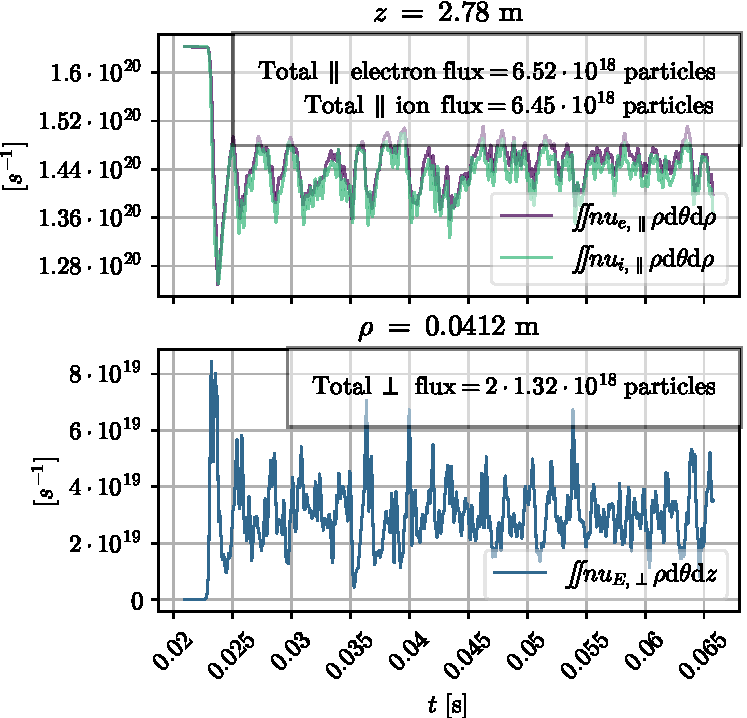
\includegraphics{fig/results/totalFlux/flux008}
    \caption{Integrated flux for $B=0.08\T$}
    \label{fig:flux008}
\end{figure}
%
In the linear phase after $0.02\s$, the radial flux is almost zero due to the small amplitudes of the fluctuations in the potential and density.
An overshoot in the energy, just like the one seen in \cref{fig:energyTrace008} follows the linear phase.
From that point in time the radial flux comes burst-wise throughout the simulation.

Although the particles are not escaping the domain in the perpendicular direction, the total perpendicular particle flux through $\mathcal{S}$
is approximately $10\%$ of the parallel flux out of the domain.
We can also observe that almost as many ions as electrons are lost in the parallel direction ($99\%$).
Physically, this means that the plasma is charging up very little over time, and that the quasi-neutrality assumtion is not broken.
